\let\negmedspace\undefined
\let\negthickspace\undefined
\documentclass[journal,12pt,twocolumn]{IEEEtran}
%\documentclass[conference]{IEEEtran}
%\IEEEoverridecommandlockouts
% The preceding line is only needed to identify funding in the first footnote. If that is unneeded, please comment it out.
\usepackage{cite}
\usepackage{amssymb,amsfonts,amsthm,amsmath}
\usepackage{algorithmic}
\usepackage{graphicx}
\usepackage{textcomp}
\usepackage{xcolor}
\usepackage{txfonts}
\usepackage{listings}
\usepackage{enumitem}
\usepackage{mathtools}
\usepackage{gensymb}

%%
%\usepackage{setspace}
%%\doublespacing
%\singlespacing
%
%%\usepackage{graphicx}
%%\usepackage{amssymb}
%%\usepackage{relsize}
%\usepackage[cmex10]{amsmath}
%%\interdisplaylinepenalty=2500
%%\savesymbol{iint}
%%\usepackage{txfonts}
%%\restoresymbol{TXF}{iint}
%%\usepackage{wasysym}
%\usepackage{amsthm}
%\usepackage{mathrsfs}
%\usepackage{txfonts}
%%\usepackage{stfloats}
%%\usepackage{cite}
%%\usepackage{cases}
%%\usepackage{subfig}
%%\usepackage{xtab}
%%\usepackage{multirow}
%%\usepackage{algorithm}
%%\usepackage{algpseudocode}
%%\usepackage{tikz}
%%\usepackage{circuitikz}
%%\usepackage{verbatim}
\usepackage{hyperref}
%%\usepackage{stmaryrd}
%%\usepackage{tkz-euclide} % loads  TikZ and tkz-base
%%\usetkzobj{all}
    \usepackage{color}                                            %%
    \usepackage{array}                                            %%
    \usepackage{longtable}                                        %%
    \usepackage{calc}                                             %%
    \usepackage{multirow}                                         %%
    \usepackage{hhline}                                           %%
    \usepackage{ifthen}                                           %%
%  %optionally (for landscape tables embedded in another document): %%
%    \usepackage{lscape}     
%%\usepackage{multicol}
%\usepackage{chngcntr}
%\usepackage{enumerate}

%\usepackage{wasysym}
%\newcounter{MYtempeqncnt}
\DeclareMathOperator*{\Res}{Res}
%\renewcommand{\baselinestretch}{2}
\renewcommand\thesection{\arabic{section}}
\renewcommand\thesubsection{\thesection.\arabic{subsection}}
\renewcommand\thesubsubsection{\thesubsection.\arabic{subsubsection}}

\renewcommand\thesectiondis{\arabic{section}}
\renewcommand\thesubsectiondis{\thesectiondis.\arabic{subsection}}
\renewcommand\thesubsubsectiondis{\thesubsectiondis.\arabic{subsubsection}}

% correct bad hyphenation here
\hyphenation{op-tical net-works semi-conduc-tor}
\def\inputGnumericTable{}                                 %%

\lstset{
language=tex,
frame=single, 
breaklines=true
}

\begin{document}
%


\newtheorem{theorem}{Theorem}[section]
\newtheorem{problem}{Problem}
\newtheorem{proposition}{Proposition}[section]
\newtheorem{lemma}{Lemma}[section]
\newtheorem{corollary}[theorem]{Corollary}
\newtheorem{example}{Example}[section]
\newtheorem{definition}[problem]{Definition}
%\newtheorem{thm}{Theorem}[section] 
%\newtheorem{defn}[thm]{Definition}
%\newtheorem{algorithm}{Algorithm}[section]
%\newtheorem{cor}{Corollary}
\newcommand{\BEQA}{\begin{eqnarray}}
\newcommand{\EEQA}{\end{eqnarray}}
\newcommand{\define}{\stackrel{\triangle}{=}}

\bibliographystyle{IEEEtran}
%\bibliographystyle{ieeetr}


\providecommand{\mbf}{\mathbf}
\providecommand{\pr}[1]{\ensuremath{\Pr\left(#1\right)}}
\providecommand{\re}[1]{\ensuremath{\text{Re}\left(#1\right)}}
\providecommand{\im}[1]{\ensuremath{\text{Im}\left(#1\right)}}
\providecommand{\qfunc}[1]{\ensuremath{Q\left(#1\right)}}
\providecommand{\sbrak}[1]{\ensuremath{{}\left[#1\right]}}
\providecommand{\lsbrak}[1]{\ensuremath{{}\left[#1\right.}}
\providecommand{\rsbrak}[1]{\ensuremath{{}\left.#1\right]}}
\providecommand{\brak}[1]{\ensuremath{\left(#1\right)}}
\providecommand{\lbrak}[1]{\ensuremath{\left(#1\right.}}
\providecommand{\rbrak}[1]{\ensuremath{\left.#1\right)}}
\providecommand{\cbrak}[1]{\ensuremath{\left\{#1\right\}}}
\providecommand{\lcbrak}[1]{\ensuremath{\left\{#1\right.}}
\providecommand{\rcbrak}[1]{\ensuremath{\left.#1\right\}}}
\theoremstyle{remark}
\newtheorem{rem}{Remark}
\newcommand{\sgn}{\mathop{\mathrm{sgn}}}
\providecommand{\abs}[1]{\left\vert#1\right\vert}
\providecommand{\res}[1]{\Res\displaylimits_{#1}} 
\providecommand{\norm}[1]{\left\lVert#1\right\rVert}
%\providecommand{\norm}[1]{\lVert#1\rVert}
\providecommand{\mtx}[1]{\mathbf{#1}}
\providecommand{\mean}[1]{E\left[ #1 \right]}
\providecommand{\fourier}{\overset{\mathcal{F}}{ \rightleftharpoons}}
%\providecommand{\hilbert}{\overset{\mathcal{H}}{ \rightleftharpoons}}
\providecommand{\system}{\overset{\mathcal{H}}{ \longleftrightarrow}}
	%\newcommand{\solution}[2]{\textbf{Solution:}{#1}}
\newcommand{\solution}{\noindent \textbf{Solution: }}
\providecommand{\dec}[2]{\ensuremath{\overset{#1}{\underset{#2}{\gtrless}}}}
\newcommand{\myvec}[1]{\ensuremath{\begin{pmatrix}#1\end{pmatrix}}}
\newcommand{\mydet}[1]{\ensuremath{\begin{vmatrix}#1\end{vmatrix}}}
	\newcommand*{\permcomb}[4][0mu]{{{}^{#3}\mkern#1#2_{#4}}}
\newcommand*{\perm}[1][-3mu]{\permcomb[#1]{P}}
\newcommand*{\comb}[1][-1mu]{\permcomb[#1]{C}}
\providecommand{\gauss}[2]{\mathcal{N}\ensuremath{\left(#1,#2\right)}}
%%
%	%\newcommand{\solution}[2]{\textbf{Solution:}{#1}}
%\newcommand{\solution}{\noindent \textbf{Solution: }}
\newcommand{\cosec}{\,\text{cosec}\,}
\newcommand{\sinc}{\,\text{sinc}\,}
\newcommand{\rect}{\,\text{rect}\,}

%\numberwithin{equation}{section}
\numberwithin{equation}{subsection}
%\numberwithin{problem}{section}
%\numberwithin{definition}{section}
\makeatletter
\@addtoreset{figure}{problem}
\makeatother

\let\StandardTheFigure\thefigure
\let\vec\mathbf
\let\j\jmath
%\renewcommand{\thefigure}{\theproblem.\arabic{figure}}
\renewcommand{\thefigure}{\theproblem}
%\setlist[enumerate,1]{before=\renewcommand\theequation{\theenumi.\arabic{equation}}
%\counterwithin{equation}{enumi}


%\renewcommand{\theequation}{\arabic{subsection}.\arabic{equation}}

\def\putbox#1#2#3{\makebox[0in][l]{\makebox[#1][l]{}\raisebox{\baselineskip}[0in][0in]{\raisebox{#2}[0in][0in]{#3}}}}
     \def\rightbox#1{\makebox[0in][r]{#1}}
     \def\centbox#1{\makebox[0in]{#1}}
     \def\topbox#1{\raisebox{-\baselineskip}[0in][0in]{#1}}
     \def\midbox#1{\raisebox{-0.5\baselineskip}[0in][0in]{#1}}

\vspace{3cm}

\title{
%	\logo{
	Probability: Assignment 1
%	}
}
%\title{
%	\logo{Matrix Analysis through Octave}{\begin{center}\includegraphics[scale=.24]{tlc}\end{center}}{}{HAMDSP}
%}


% paper title
% can use linebreaks \\ within to get better formatting as desired
%\title{Matrix Analysis through Octave}
%
%
% author names and IEEE memberships
% note positions of commas and nonbreaking spaces ( ~ ) LaTeX will not break
% a structure at a ~ so this keeps an author's name from being broken across
% two lines.
% use \thanks{} to gain access to the first footnote area
% a separate \thanks must be used for each paragraph as LaTeX2e's \thanks
% was not built to handle multiple paragraphs
%

\author{
	Sree Anusha Ganapathiraju\\
	CC22RESCH11003
	%<-this % stops a space
%\thanks{}}
}
\maketitle

\newpage

\tableofcontents

\bigskip

\renewcommand{\thefigure}{\theenumi}
\renewcommand{\thetable}{\theenumi}

		\numberwithin{equation}{enumi}
\section{Uniform Random Numbers}
Let $U$ be a uniform random variable between 0 and 1.
\begin{enumerate}[label=\thesection.\arabic*
,ref=\thesection.\theenumi]
\item Generate $10^6$ samples of $U$ using a C program and save into a file called uni.dat .
\\
\solution Download the following files and execute the  C program.
\begin{lstlisting}
Assignment 1/codes/exrand.c
Assignment 1/codes/coeffs.h
\end{lstlisting}

%
\item
Load the uni.dat file into python and plot the empirical CDF of $U$ using the samples in uni.dat. The CDF is defined as
\begin{align}
F_{U}(x) = \pr{U \le x}
\end{align}
\\
\solution  The following code plots Fig. \ref{fig:uni_cdf}
\begin{lstlisting}
Assignment 1/codes/cdf_plot.py
\end{lstlisting}

\begin{figure}
\centering
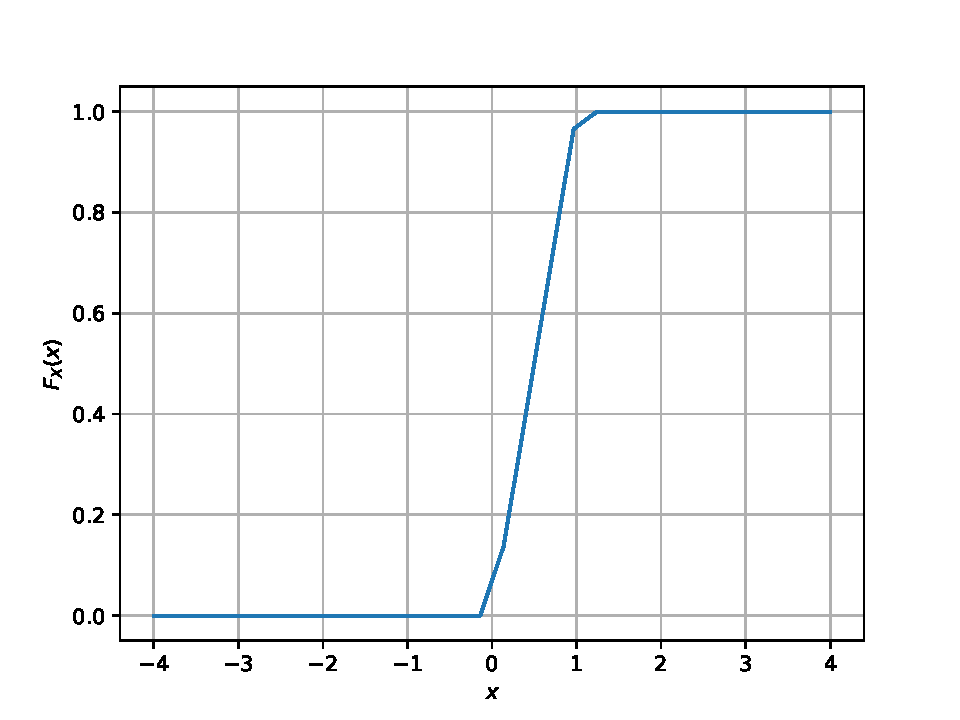
\includegraphics[width=\columnwidth]{./figs/uni_cdf}
\caption{The CDF of $U$}
\label{fig:uni_cdf}
\end{figure}

%
\item
Find a  theoretical expression for $F_{U}(x)$.\\
\solution
The Probaility Density Function for Uniform Distribution is given by:\\
\begin{equation}
  f(x) =
    \begin{cases}
      1 & x\in [0,1]\\
      0 & \text{Otherwise}
    \end{cases}       
\end{equation}

The Cumulative Distribution Function is defined by 
\begin{equation*}
F_{U}(x)=\int_{-\infty}^{x}f(x)dx
\end{equation*}
So, we can split in for three intervals, as\\
\begin{equation*}
F_{U}(x)=\int_{-\infty}^{0}f(x)dx+\int_{0}^{1}f(x)dx+\int_{1}^{\infty}f(x)dx
\end{equation*}
Accordingly, we have three cases as follows:\\
Case 1: 
\begin{equation*}
\int_{-\infty}^{0}f(x)dx
\end{equation*} if $x<0$ then,$f(x)=0$ and but $\lim_{x\to\infty} F(x)=0$\\
Case 2: 
\begin{equation*}
\int_{0}^{1}f(x)dx
\end{equation*} if $0\leq x\leq 1$ then, 
\begin{equation*}
\int_{0}^{1}f(x)dx=\frac{1}{1-0}\int_{0}^{1}dx=\left[\frac{x}{1-0}\right]_{0}^{1}=1
\end{equation*}\\
Case 3: 
\begin{equation*}
\int_{1}^{\infty}f(x)dx
\end{equation*} if $x>b$ then, $f(x)=0$ but $\lim_{x\to\infty} F(x) =1$ \\Thus, The Cumulative Distribution for uniform random variable is given as follows:
\begin{equation}
  F_{U}(x)=\pr{U \le x} =
    \begin{cases}
    0 & \text{for x $<$ 0}\\
      \frac{x-0}{1-0} & x\in [0,1]\\
      1 & \text{for x $>$ 1}
    \end{cases}       
\end{equation}
\item
The mean of $U$ is defined as
%
\begin{equation}
E\sbrak{U} = \frac{1}{N}\sum_{i=1}^{N}U_i
\end{equation}
%
and its variance as
%
\begin{equation}
\text{var}\sbrak{U} = E\sbrak{U- E\sbrak{U}}^2 
\end{equation}
Write a C program to  find the mean and variance of $U$. \\
\solution
The C Program is executed in the following
\begin{lstlisting}
Assignment 1/codes/exrand.c
Assignment 1/codes/coeffs.h
\end{lstlisting}
The mean value is \textbf{0.50} and variance value is \textbf{0.083}\\
\item Verify your result theoretically given that
\begin{equation}
E\sbrak{U^k} = \int_{-\infty}^{\infty}x^kdF_{U}(x)
\end{equation}
\end{enumerate}
\solution
Mean is given by $E[U]=\int_{0}^{1}xdF_{U}(x)$
Accordingly,
\begin{align*}
& E[U]=\int_{0}^{1}xdF_{U}(x)
\\
& =\int_{0}^{1}x dx
\\
& =\left[\frac{x^2}{2}\right]_0^{1}
\\
& =\frac{1}{2}=0.50
\end{align*}
Now, for $E[U^2]$, we have,
\begin{align*}
& E[U^2]=\int_{0}^{1}x^2dF_{U}(x)
\\ 
& =\int_{0}^{1}x^2 dx
\\
& =\left[\frac{x^3}{3}\right]_0^{1}
\\
& =\frac{1}{3}
\end{align*}
Now, we know from \textbf{1.4} that, 
\begin{align*}
& \text{var}\sbrak{U} = E\sbrak{U- E\sbrak{U}}^2
\\
& =E[U^2-2UE[U]+(E[U])^2]
\\
&  =E[U^2]-2E[U]E[U]+E[E[U]^2]
\\
& =E[U^2]-2E[U]^2+E[U]^2
\\
& = E[U^2]-E[U]^2
\end{align*}
Substituting the Values for $E[U]$ and $E[U^2]$ in the above equation, we get, \\
\begin{align*}
& \text{var}[U]=\frac{1}{3}-\left(\frac{1}{2}\right)^2
\\
& \frac{1}{3}-\frac{1}{4}=\frac{1}{12}=0.083
\end{align*}
Hence Proved.


\end{document}
